\chapter{技術記事のまとめ}

\begin{itemize}
      \item suda \\
            p.7 『DiscordBot を作ってみよう』 \\
            似たような会話をするのが煩わしいので自分っぽい反応をするDiscordBotを作ってみました! \\
      \item hihumikan \\
            p.11『リポジトリ作成後に設定しておきたいこと』 \\
            Git初心者に向けたGitで使えると嬉しいことをまとめました! \\ 
      \item 水谷 \\
            p.16『Gin × Neo4j × Docker で最短経路を返す API サーバを建てる』 \\
            グラフDBであるNeo4jとGo(Gin)を用いた経路探索APIと、そのAPIサーバを構築します!! \\
      \item Beyond Toyama \\
            p.29『Next.js 13 触ってみた』 \\
            最新のNext.js 13になったことで追加された機能や変更された部分を紹介しています! \\
\end{itemize} 

% \begin{figure}[H]
%   \centering
%   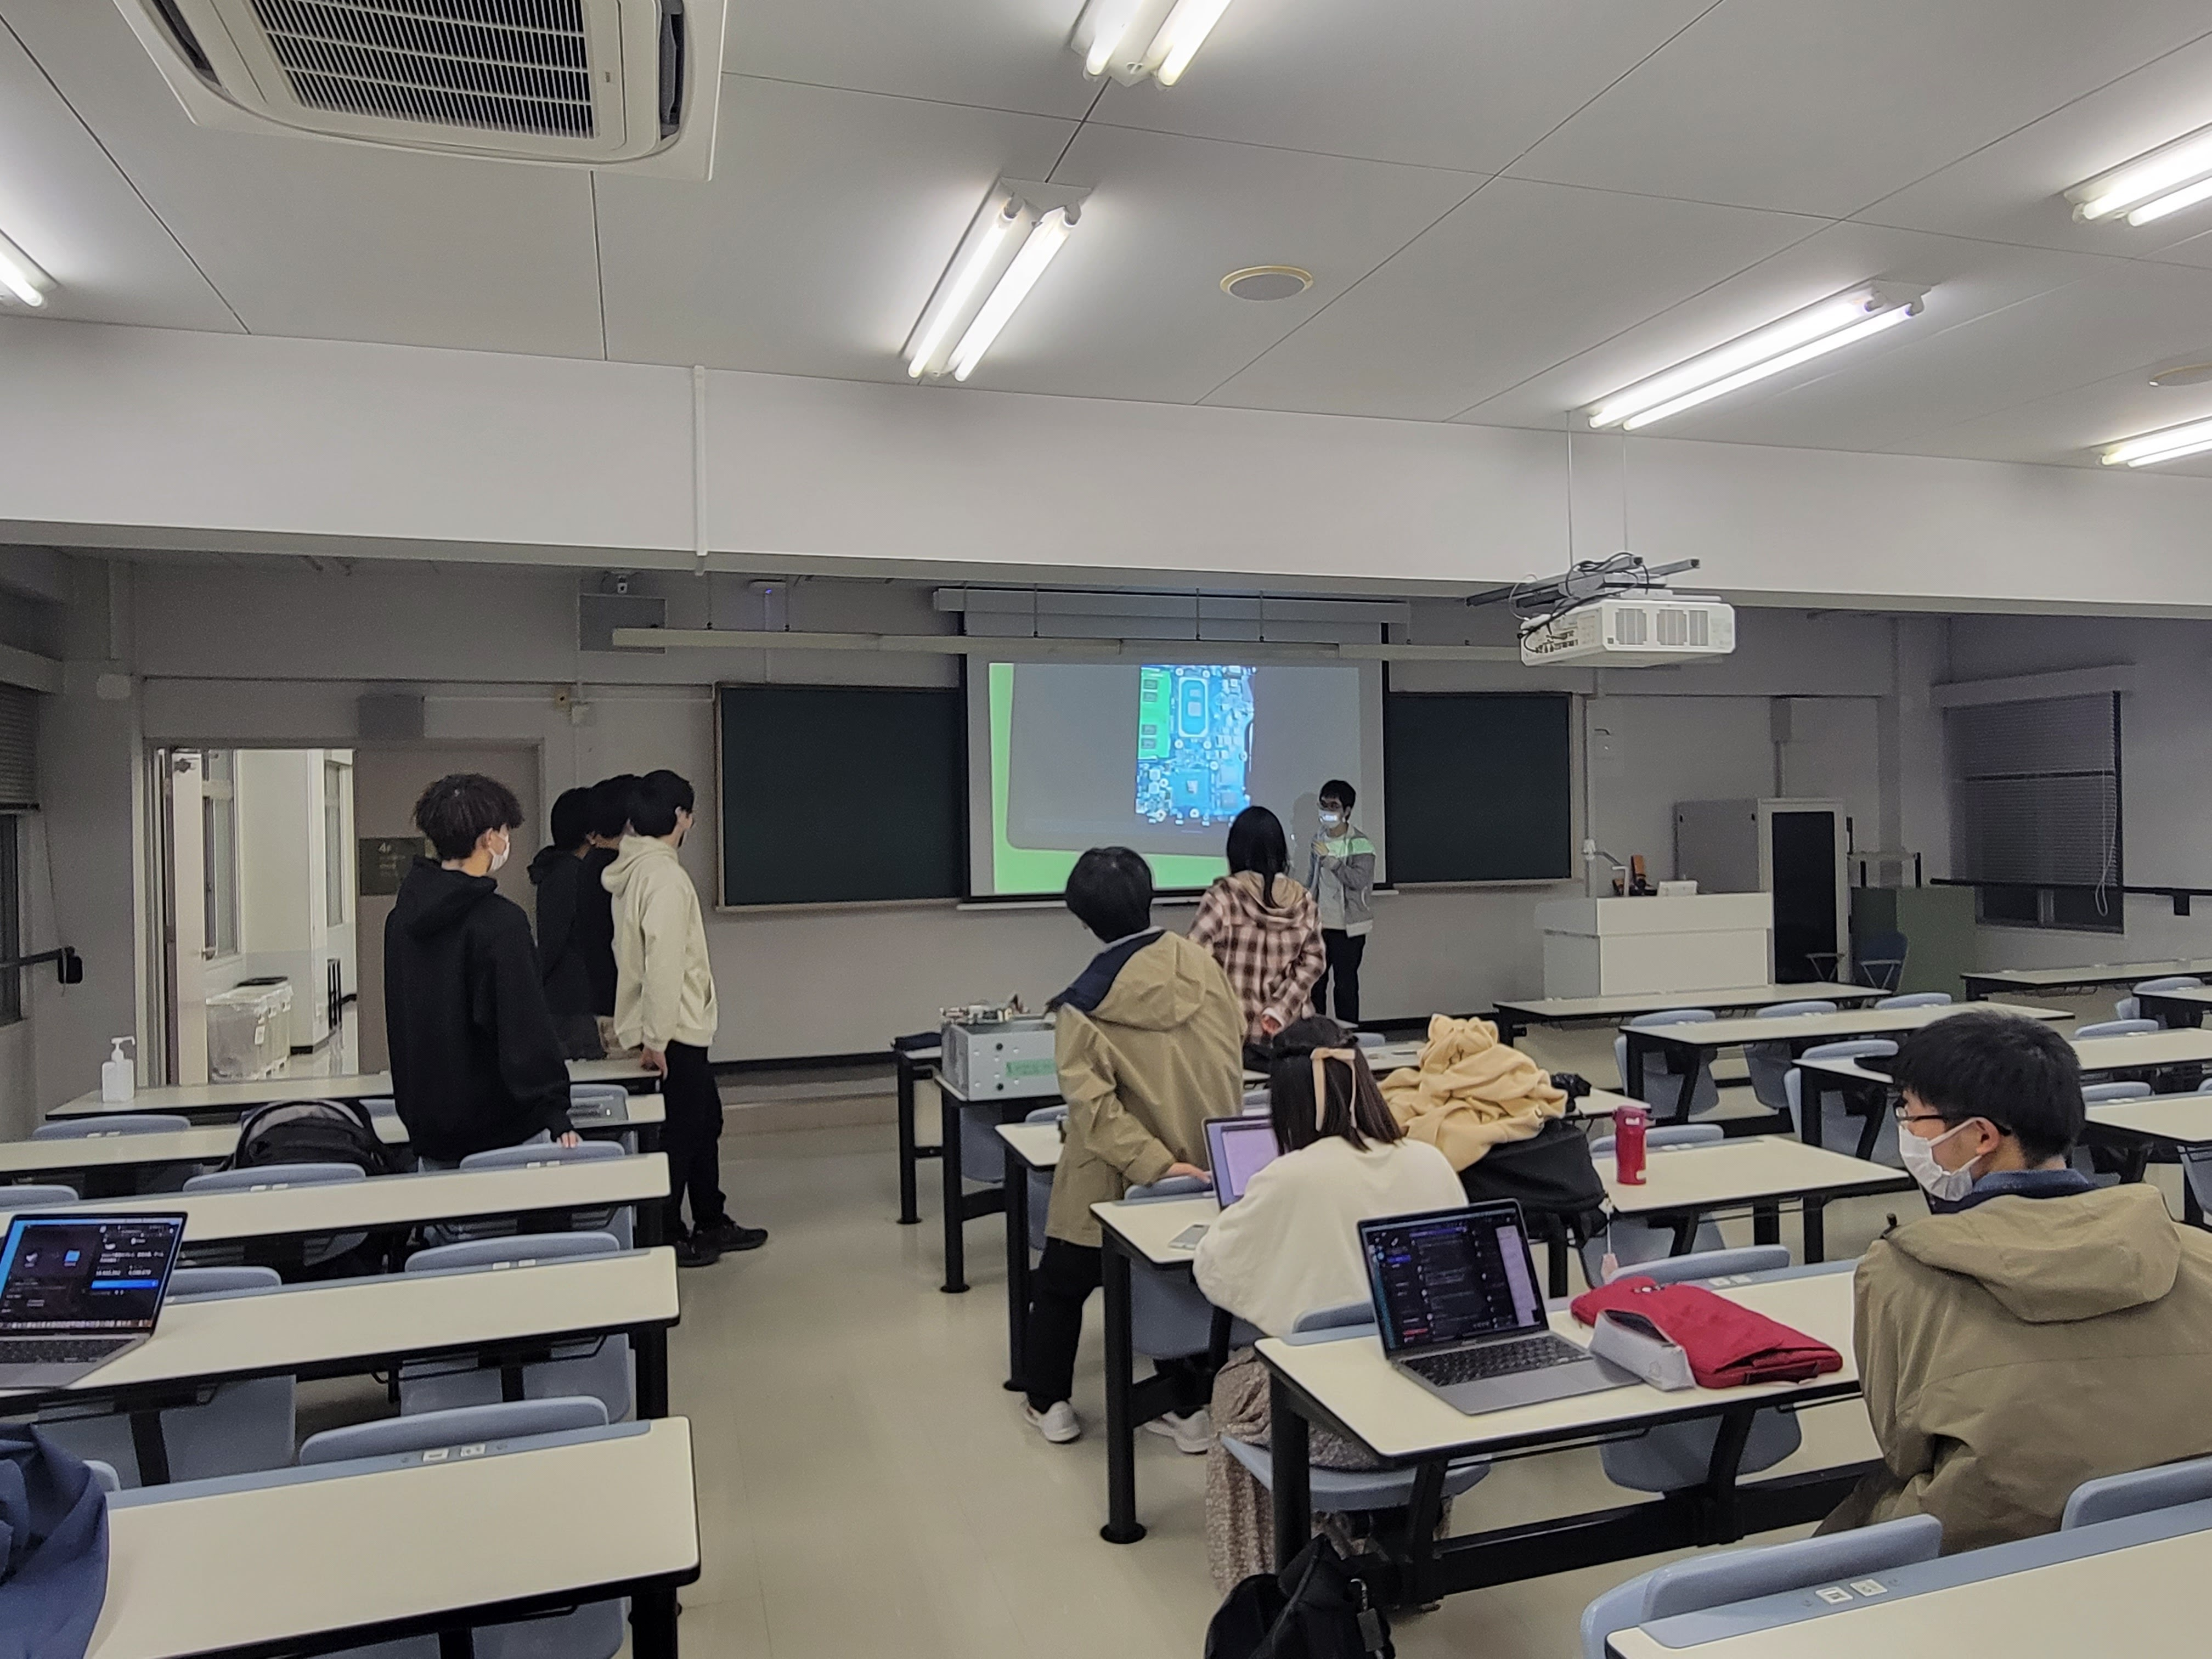
\includegraphics[width=6cm]{./image/03-Tech/benkyoukai.jpg}
%   \caption{シス研で勉強会を行っている様子}
%   \label{benkyoukai}
% \end{figure}